\chapter{The Standard Model of Particle Physics}

Ever since Democritus' philosophy of atomism, one of the driving desires behind mankind's advancements in the fields of natural science has been to reduce reality to its basic components.

[...], this chapter explores the theoretical framework for the rest of thesis, introducing key concepts such as \textit{spin}, \textit{helicity} and the importance of \textit{angular distributions} of decay products.

\section{Elementary particles}
\begin{figure}[t!]
	\centering
	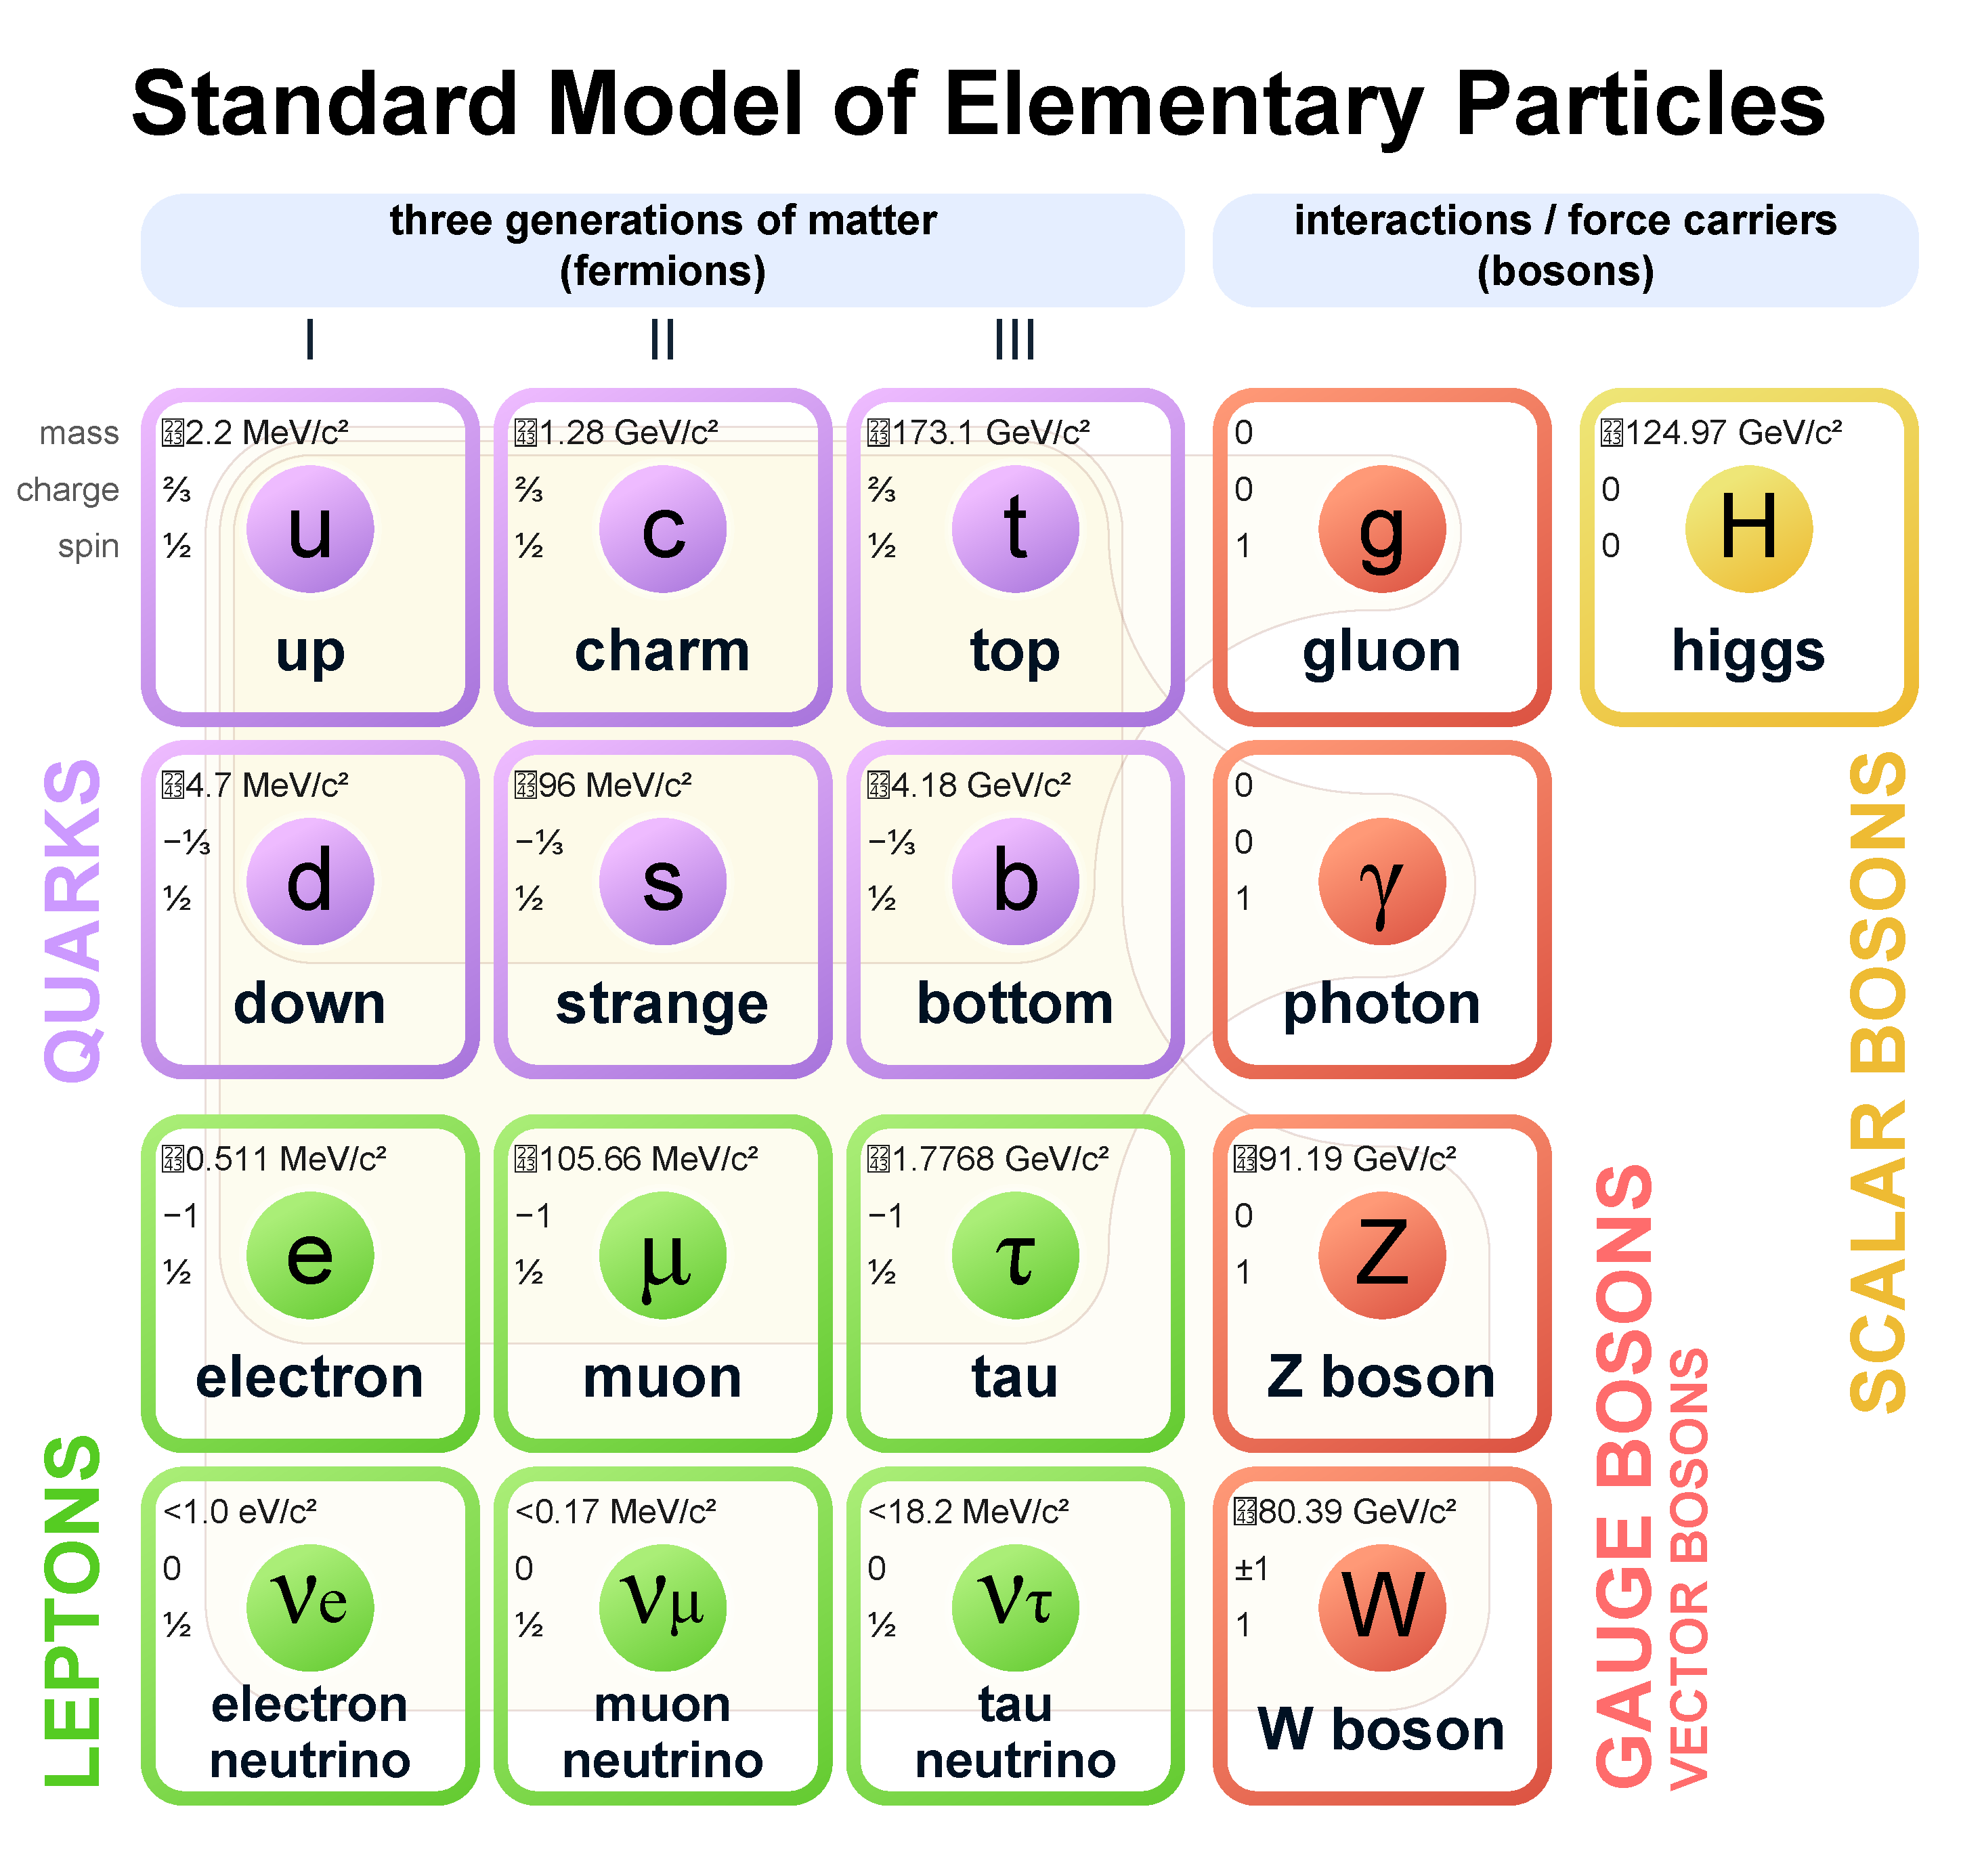
\includegraphics[scale=0.15]{graphics/01-standard_model/Standard_Model_of_Elementary_Particles.pdf}
	\caption[Currently known Standard Model elementary particles.]{The seventeen currently known elementary particles of the Standard Model. Antiparticles are not depicted.}
	\label{fig:particle_zoo}
\end{figure}

Intuitively, a particle is said to be \textit{elementary} when it displays no substructure that we know of. 
A century of efforts in the fields of nuclear, quantum, and high energy physics has whittled down the spectrum of matter to just seventeen unique fundamental particles, colloquially known as the \textit{particle zoo} and depicted in Figure \ref{fig:particle_zoo}.

Each of the ten charged particles is joined by an \textit{antimatter particle} (\textit{antiparticle} for short), a companion of opposite charge identified by the prefix \textit{anti-}, e.g. antimuon for the muon; the only exception to this naming convention is the electron, whose antiparticle, for historical reasons, is known as positron. While often omitted for the sake of brevity, antiparticles are elementary particles in every respect, distinct from their partners and related to them through the transformation of \textit{charge conjugation}.

\subsection{Leptons}
Fermioni.

\subsection{Quarks}
Adroni, mesoni e barioni. QCD. Storia della scoperta. Tre colori.

%% Questa è scritta proprio male.
Unlike leptons, quarks are impossible to observe directly: according to the phenomenon of \textit{color confinement}, the energy of the interaction field between two color charges being pulled apart increases until it becomes high enough to create a quark-antiquark pair. This process of \textit{fragmentation} develops many times over in such a way that the final observable state is entirely composed of colorless particles. For this reason, high energy physics experiments such as LHCb do not detect free quarks, instead observing cone-shaped streams of hadrons known as \textit{hadronic jets}.

\subsection{Gauge bosons and fundamental interactions}
Gruppo di simmetria, principio di gauge, QCD e teoria elettrodebole.

\subsection{The Higgs boson}
Rottura spontanea della simmetria.

\section{Spin}
Spin ed EM dipole.

\section{Discrete symmetries}
CPT, violazione di CP.

\section{Helicity formalism}
Il Richman.